%% Diego Aranha
%%

\NomeDoProblema{Ludo}%
\Conceitos{Ad-Hoc}%
\Dificuldade{1}%

Um jogo simples jogado por gerações de crianças consiste em um tabuleiro contendo
uma trilha de quadrados e um conjunto de peças coloridas. No começo do jogo, cada
jogador recebe uma peça e todas as peças são inicialmente posicionadas antes do
primeiro quadrado da trilha.

O jogo prossegue em rodadas. Em cada rodada, jogadores lançam um par de dados e
avançam suas peças em um número correspondente de casas. A ordem de lançamento
dos dados é sempre a mesma (jogador $A$, jogador $B$, etc.), independente do
número da rodada.

A maioria das casas no tabuleiro são casas simples, mas três delas são casas de
armadilhas. Se a peça de um jogador cai em uma casa de armadilha ao final de sua
jogada, sua vez é pulada na próxima rodada. Ou seja, o jogador não lança os
dados e sua peça permanece na mesma casa até o fim daquela rodada.

% \vspace{0.5cm}%
\begin{figure}[h]%
	\begin{center}%
		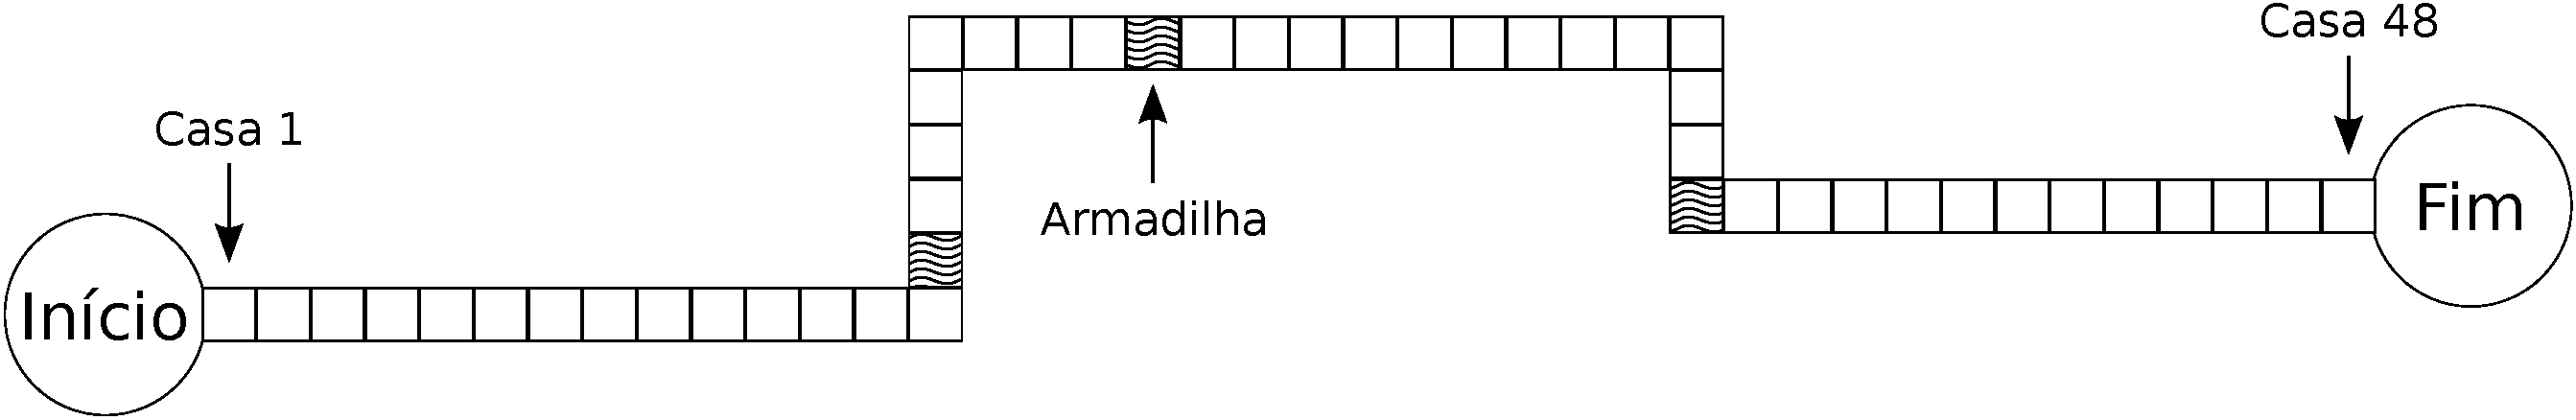
\includegraphics[scale=0.35]{tabuleiro}%
	\end{center}%
\end{figure}%

O vencedor é o jogador cuja peça atinge o final da trilha primeiro. O fim da
trilha é após a última casa do tabuleiro. Considere, por exemplo, o tabuleiro na
figura acima, que possui casas numeradas de 1 a 48. Inicialmente, as peças são
posicionadas em uma casa marcada ``Início'', antes da casa número 1.
Posteriormente, se um jogador lança o valor 7, sua peça será posicionada na
casa de número 7 ao final da primeira rodada do jogo. Se a peça futuramente
estiver posicionada na casa 41, o jogador precisa lançar um valor de pelo menos
8 para alcançar o fim da trilha e vencer o jogo. Observe também que não há
possibilidade de empate.

Neste problema, você receberá o número de jogadores, o número de casas na
trilha, a localização das armadinhas e uma lista de lançamento de dados. Você
deve escrever um programa que determina quem é o vencedor.

\Entrada%
Seu programa deve processar vários casos de teste. A primeira linha de um caso
de teste contém dois inteiros $P$ e $S$ representando respectivamente o número
de jogadores e o número de casas na trilha ($1 \leq P \leq 10$ e $3 \leq S \leq 10000$).
A segunda linha descreve as armadilhas, representadas por três inteiros distintos
$A_1, A_2$ e $A_3$ denotando suas posições na trilha ($1 \leq A_1, A_2, A_3 \leq S$).
A terceira linha contém um único inteiro $N$ indicando o número de lançamentos
de dados no caso de teste. Cada uma das $N$ linhas
seguintes contém dois inteiros $D_1$ e $D_2$ ($1 \leq D_1, D_2 \leq 6$)
representando os resultados dos lançamentos. O fim da entrada é indicado por
$P = S = 0$. O número $N$ em um teste será sempre necessário para um jogador
vencer a partida. Cada jogador é identificado por um número entre 1 e $P$. A
ordem de jogadas em uma rodada é de 1 a $P$.

\Saida%
Seu programa deve imprimir um único inteiro: o número do jogador vencedor.

\Exemplos{13,101}%
